% TESSERA - SOICT submission (Springer LNCS format)
\documentclass[runningheads]{llncs}

\usepackage[T1]{fontenc}
\usepackage{graphicx}
\usepackage{amsmath,amssymb,amsfonts}
\usepackage{booktabs}
\usepackage{enumitem}
\usepackage{bm}
\usepackage{mathtools}
\usepackage{xcolor}

% ─── Notation shorthands ─────────────────────────────────────────────────────
\newcommand{\R}{\mathbb{R}}
\newcommand{\OUV}{\Omega_{\text{UV}}}
\newcommand{\Oin}{\Omega_{\text{in}}}
\newcommand{\Vis}{\operatorname{Vis}}
\newcommand{\Tpartial}{T_{\text{partial}}}
\newcommand{\Tcomplete}{T_{\text{complete}}}
\newcommand{\cM}{\mathcal{M}}
\newcommand{\Rel}{\mathcal{R}}
% Placeholder for values NOT YET MEASURED - shown in red so they cannot be missed
\newcommand{\PH}[1]{\textcolor{red}{#1}}


\begin{document}

\title{TESSERA: Self-Estimated Reliability Arbitration for
Complete-Texture Free-Viewpoint Face Avatars from a Single Image}
\titlerunning{TESSERA: Reliability Arbitration for Face Texture Completion}

% TODO: fill in author and affiliation before submission
\author{\PH{First Author}\inst{1} \and \PH{Second Author}\inst{1}}
\authorrunning{\PH{F. Author et al.}}
\institute{\PH{Affiliation, City, Country}\\
\email{\PH{email@domain}}}

\maketitle

% Ban thao: moi gia tri mau do (\PH) la so CHUA DO. Xoa macro mau khi nop.

% ─────────────────────────────────────────────────────────────────────────────
\begin{abstract}
Monocular 3D face reconstruction recovers accurate geometry from a single
image, but its texture is baked from one viewpoint: surfaces occluded at
capture receive no observation, leaving much of the UV atlas undefined and the
reconstructed mesh unusable for free-viewpoint rendering. The prevailing remedy
delegates the atlas to a generative model. We argue this concedes too much---a
generative prior re-synthesizes even the regions that \emph{were} directly
observed, discarding real photometric evidence of the subject, and it reports
nothing about which texels can be trusted.
We recast texture completion as \emph{arbitration among evidence sources of
differing reliability}. Our key observation is that every source can estimate
its own reliability from a residual it must compute anyway: cross-topology
transport from surface distance and normal agreement, symmetry transport from
the asymmetry residual measured where both halves are observed, and the
generative prior from the variance across repeated samples. Because the three
estimates share a common scale, they are fused by a single reliability-anchored
Poisson solve on a texel graph that follows surface connectivity rather than the
UV plane. TESSERA therefore consults the generative prior \emph{last} rather
than first.
The completed atlas carries its own reliability field, which predicts rendering
quality at any camera pose before rendering. On V-Face
(\PH{74} subjects, seven calibrated views spanning $\pm90^\circ$ yaw), TESSERA
improves \PH{[PSNR/SSIM/LPIPS/CSIM]} over a contemporary UV diffusion prior
applied to the same task, and its predicted reliability correlates with measured
per-view quality at \PH{[r]}.
\keywords{Face texture completion \and Evidence fusion \and Reliability
estimation \and Cross-topology texture transfer \and Free-viewpoint rendering
\and Single-image face avatar}
\end{abstract}

% ─────────────────────────────────────────────────────────────────────────────
\section{Introduction}

Three-dimensional face avatars reconstructed from ordinary photographs are used
in telepresence, digital content production and cultural heritage
applications. In all of these settings the avatar is rendered from viewpoints
other than the one at which it was captured, which requires an appearance
representation defined over the entire head surface.

Monocular reconstruction methods recover facial geometry from a single image
with high accuracy \cite{paysan2009bfm,feng2021deca}, but their appearance
output is obtained by projecting the input image onto the reconstructed
surface, so only the regions visible to the capture camera receive a valid
observation. The remaining regions, typically the contralateral cheek, the ear
and part of the jaw, are either left undefined or filled by interpolation from
distant texels. This is not an occasional failure but a deterministic
consequence of the capture geometry: at a lateral capture angle of
$30^{\circ}$, \PH{40--58\%} of the UV atlas receives no observation.

The established remedy is to complete the atlas with a generative prior trained
in UV space \cite{rombach2022ldm,li2024uvidm}. This restores coverage, but
delegating the entire atlas to a generative model introduces two limitations
that have not been examined. First, the model re-synthesizes the regions that
were directly observed, so photometric evidence of the specific subject is
replaced by content that is only statistically plausible; we measure a
consistent loss of high-frequency detail there. Second, the completed atlas is
returned without any indication of which texels are supported by observation
and which were inferred, so every subsequent stage treats all texels as equally
reliable. A further difficulty is practical: the prior and the animation model
rarely share a mesh topology, so the atlas must be transferred between two UV
parameterizations before it can be used.

We reformulate texture completion as the arbitration of several sources of
evidence that differ in reliability. Our central observation is that each
source can estimate its own reliability from a residual it must compute in any
case. Transporting the observed texture across the topology gap yields a
surface distance and a normal agreement at every texel; mirroring the observed
half of the face onto the occluded half yields an asymmetry residual on the
region where both halves are observed; and sampling the generative prior
repeatedly yields a per-texel variance. These quantities require no additional
supervision and no manually tuned thresholds, and share a common scale, which
allows the corresponding evidence to be combined in a single optimization
rather than selected by hard masks.

We present TESSERA, which ranks evidence by self-estimated reliability and
consults the generative prior last rather than first. Observed texels are
preserved, occluded texels are recovered from the mirrored observation of the
same subject wherever the estimated symmetry supports it, and the prior
supplies only the remainder; the three are merged by one reliability-anchored
Poisson solve on a texel graph that follows surface connectivity rather than
the UV layout. The method requires a single image and no per-subject
optimization, in contrast to representations optimized separately for each
subject from video \cite{qian2024gaussianavatars}.

\medskip\noindent\textbf{Contributions.}
\begin{itemize}[leftmargin=*,nosep]
\item We replace the binary notion of UV coverage with a continuous reliability
  field, of which the binary condition is the degenerate case.
\item We show that geometric transport, symmetry transport and a generative
  prior can each report their reliability from a residual they already compute,
  on a common scale and without additional training, and we introduce an
  intrinsic symmetry transport that recovers occluded regions from observations
  of the same subject rather than from generated content.
\item We merge the evidence with a single reliability-anchored Poisson problem
  on a texel graph that follows surface connectivity across UV cuts, replacing
  the morphological operations used by prior pipelines.
\item We derive a per-viewpoint quality estimate from the reliability field and
  evaluate it, with the completed textures, on \PH{74} subjects across seven
  calibrated viewpoints spanning $\pm 90^{\circ}$ of yaw.
\end{itemize}

\section{Related Work}

\textbf{Monocular face reconstruction.} Recovering facial geometry from
unconstrained images is commonly formulated on top of a 3D morphable model
\cite{blanz1999morphable}, refined by the Basel Face Model
\cite{paysan2009bfm} and by FLAME \cite{li2017flame}, which separate identity
shape from expression through linear bases. Regression architectures such as
DECA \cite{feng2021deca} predict these parameters from a single image and
produce animation-ready meshes without per-subject fitting. Their appearance
branch is not designed for completeness: it either samples a low-dimensional
albedo prior or projects the visible pixels onto the mesh, and in both cases
the regions occluded at capture remain unsupported. We use such a method as the
geometry backbone, and the incompleteness of its baked texture defines the
problem addressed here.

\textbf{Generative texture completion in UV space.} To fill unobserved regions,
recent work applies generative priors directly in the UV domain. Following
latent diffusion models \cite{rombach2022ldm}, UV-IDM \cite{li2024uvidm}
synthesizes identity-conditioned appearance over the full atlas. These models
produce plausible content and restore coverage, and we adopt one of them as a
component. Our departure concerns how the generated content is used: existing
pipelines pass the entire atlas through the generative model and accept its
output uniformly, whereas we treat it as the least reliable of several sources
of evidence and consult it only where no observation, direct or symmetric, is
available.

\textbf{Monocular avatar representations.} A parallel line of work reconstructs
renderable head avatars by optimizing a neural or point-based representation
separately for each subject from a monocular video
\cite{gafni2021nerface,grassal2022nha,qian2024gaussianavatars,zhang2025fate}.
These methods reach high rendering fidelity and can represent
expression-dependent appearance, which an explicit static atlas does not, but
they require a video of the subject and a per-subject optimization stage,
whereas our method takes a single image and outputs an explicit atlas on a
shared animation topology. We therefore regard them as complementary rather
than directly comparable, and compare quantitatively only against methods that
operate from a single image. For evaluation we use the V-Face database
\cite{duong2022vface}, which provides multi-view captures of the same identity
and therefore ground truth for viewpoints that are never observed.

\section{Method}

\subsection{Problem Setting and the Reliability Field}
\label{sec:setting}

A monocular reconstruction method maps an input image $\mathbf{I}$ to a mesh
with vertices $\mathbf{V} \in \R^{N \times 3}$ and a fixed topology shared
across subjects \cite{li2017flame,feng2021deca}. The mesh carries a UV
parameterization $\varphi\colon \OUV \to \mathcal{S}$ over $\OUV = [0,1]^2$,
and a camera with pose $\bm{\theta}_p$ projects the surface by
$\pi(\cdot\,;\bm{\theta}_p)$. Appearance is obtained by projecting the image
onto the surface,
\begin{equation}
  \Tpartial(u,v) =
  \begin{cases}
    \mathbf{I}\bigl(\pi(\varphi(u,v);\bm{\theta}_p)\bigr)
      & \varphi(u,v) \in \Vis(\bm{\theta}_p),\\[2pt]
    \text{undefined} & \text{otherwise},
  \end{cases}
  \label{eq:baking}
\end{equation}
where $\Vis(\bm{\theta}_p)$ is the set of surface points visible at capture and
$\Oin$ denotes the observed part of the atlas.

Prior formulations treat completeness as binary: a texel is either observed or
not. This is too coarse for a completed atlas, in which texels differ widely in
how well they represent the subject. A texel filled by a generative model, one
recovered from the mirrored side of the same face, and one observed at a
grazing angle are all covered, yet support rendering to very different degrees.
We therefore replace $\Oin$ with a \emph{reliability field}
\begin{equation}
  \Rel\colon \OUV \to [0,1],
  \label{eq:reliability_def}
\end{equation}
where $\Rel(u,v)$ expresses the expected agreement between the completed
texture and the true appearance of the subject at that texel. The binary
condition is the degenerate case $\Rel = \mathbf{1}_{\Oin}$. The field is not
an auxiliary diagnostic: it determines how the available evidence is combined
and it predicts the quality attainable at a given viewpoint.

\begin{figure}[htbp]
  \centering
  
\includegraphics[width=0.66\textwidth]{overview.png}
  \caption{Overview of TESSERA. Three evidence sources are transported into the
       target atlas, each reporting a reliability derived from its own
       residual; one reliability-anchored Poisson solve merges them into a
       completed atlas and its reliability field.}
  \label{fig:overview}
\end{figure}

TESSERA treats completion as arbitration among three sources of evidence
(Fig.~\ref{fig:overview}), each expressed in the target atlas as a pair
$(E_k, \Rel_k)$ of an evidence image and a reliability map: the directly
observed texture of Eq.~\eqref{eq:baking}; the observation of the mirrored half
of the face, transported through the estimated intrinsic symmetry of the
subject; and a generative UV prior, transported across the topology gap. Each
reliability comes from a residual that its branch computes in the course of its
own operation, so no additional supervision and no manually chosen thresholds
are needed, and because they share a scale the sources are combined by a single
optimization rather than selected by disjoint masks.

\subsection{Evidence Transport and Self-Estimated Reliability}
\label{sec:evidence}

\textbf{Direct observation.} The backbone bakes $\Tpartial$ in the
parameterization of the animation mesh, so the direct evidence requires no
transport: $E_{\text{dir}} = \Tpartial$. Its reliability reflects the quality
of the observation rather than its mere existence,
\begin{equation}
  \Rel_{\text{obs}}(u,v) = V(u,v)\;\cos\alpha(u,v)\;\eta(u,v),
  \label{eq:r_obs}
\end{equation}
where $V$ is binary visibility, $\alpha$ is the angle between the surface
normal and the viewing direction, and $\eta$ is the texel-to-pixel sampling
density. A texel seen at a grazing angle is observed, but its evidence is
weaker than that of a texel seen frontally; Eq.~\eqref{eq:r_obs} makes this
explicit, whereas a binary mask cannot.

\textbf{Cross-topology transport.} Generative UV priors use their own mesh and
UV layout, so the same coordinate $(u,v)$ denotes different surface points in
the two parameterizations. We therefore construct a dense transport map
$\Phi\colon \OUV^{\text{tgt}} \to \OUV^{\text{src}}$. The source mesh is
registered to the target by a landmark-based similarity transform followed by
iterative closest point refinement \cite{besl1992icp}
(Section~\ref{sec:impl}). For each target texel we obtain its surface point
$\mathbf{x}(u,v) = \varphi_{\text{tgt}}(u,v)$ by barycentric interpolation,
query the closest point $\mathbf{c}(u,v)$ on the registered source surface, and
read the source coordinate there, giving $\Phi(u,v)$ and the evidence
$E_{\text{gen}} = T_{\text{src}} \circ \Phi$.

Resolving $\Phi$ at texel resolution rather than at the vertices is essential:
sampling the source at the $N$ vertices and interpolating across triangles
limits the transported signal to $N$ independent values, a reduction of more
than two orders of magnitude for the meshes used here, which removes precisely
the high-frequency content the prior supplies. The registration residual is
available at every texel and yields the geometric reliability
\begin{equation}
  \Rel_{\text{geo}} =
    \Bigl[1 - \tfrac{d}{d_\tau}\Bigr]_0^1 \cdot
    \Bigl[\tfrac{\langle \hat{\mathbf{n}}_{\text{tgt}},
      \hat{\mathbf{n}}_{\text{src}}\rangle - t_0}{1 - t_0}\Bigr]_0^1,
  \label{eq:r_geo}
\end{equation}
where $d = \|\mathbf{x} - \mathbf{c}\|$, $[\cdot]_0^1$ denotes clipping,
$d_\tau$ is a scale set from the distribution of $d$ over the atlas, and $t_0$
places the zero of the normal term at the angle beyond which corresponding
surfaces face away from each other. No texel is discarded: a large residual
lowers the reliability of the transported evidence instead of removing it,
which is what allows the fusion to remain well posed everywhere.

\textbf{Intrinsic symmetry transport.} A face observed from a lateral pose
leaves one side occluded while the corresponding region on the other side is
observed; since faces are approximately bilaterally symmetric, that occluded
region admits evidence originating from the subject rather than from a
generative model. We estimate the intrinsic symmetry plane $\mathcal{P}$ of the
reconstructed geometry by minimizing the discrepancy between the mesh and its
reflection, initialized from the midline landmarks; estimating $\mathcal{P}$
from the geometry rather than assuming a coordinate plane keeps the
construction valid under arbitrary head pose. The plane induces a map
$\sigma\colon \OUV \to \OUV$ sending a texel to its counterpart on the opposite
side.

Bilateral symmetry is only approximate, so a transported observation must be
corrected. On the region $\Omega_{\text{both}} = \Oin \cap \sigma(\Oin)$
observed on both sides we estimate a smooth multiplicative correction
$\mathcal{C}$ by
\begin{equation}
  \mathcal{C} = \arg\min_{\mathcal{C} \in \mathcal{F}}
    \bigl\| E_{\text{dir}} - \mathcal{C}\cdot(E_{\text{dir}} \circ \sigma)
    \bigr\|^2_{\Omega_{\text{both}}},
  \label{eq:asym_correction}
\end{equation}
where $\mathcal{F}$ restricts $\mathcal{C}$ to low spatial frequencies, so
illumination and skin-tone differences between the two sides are absorbed while
genuine detail is preserved, giving
$E_{\text{sym}} = \mathcal{C}\cdot (E_{\text{dir}} \circ \sigma)$. The residual
of Eq.~\eqref{eq:asym_correction} is itself informative: it measures how far
bilateral symmetry holds for this particular subject. Writing $r$ for that
residual propagated along the surface from $\Omega_{\text{both}}$, we set
$\Rel_{\text{sym}} = \exp(-r^2/2\tau_{\text{sym}}^2)$. A subject whose sides
agree closely obtains high reliability for this branch; one with pronounced
asymmetry obtains low reliability and the fusion falls back on the generative
prior. The trade-off is resolved per subject from measurement, not by a fixed
weight.

\textbf{Generative prior and its uncertainty.} Where neither direct nor
symmetric evidence is available, appearance must be inferred. We use a UV-space
diffusion prior \cite{li2024uvidm} conditioned on $\Tpartial$ and its validity
mask. Such a model is normally queried once and its output accepted uniformly.
Instead we draw $k$ samples with independent noise and use their mean as the
evidence and their per-texel variance $s^2$ as an uncertainty estimate,
\begin{equation}
  \Rel_{\text{gen}} = \exp\!\left(-\frac{s^2}{2\tau_{\text{gen}}^2}\right).
  \label{eq:r_gen}
\end{equation}
Regions where the model reproduces the same content across samples are
constrained by its prior; regions where the samples disagree are regions in
which it is effectively guessing. This gives a notion of confidence for a
black-box generative component at no training cost. Because the prior is
defined in the source parameterization, this branch is transported by $\Phi$
and its reliability is $\Rel_{\text{gen}}\cdot\Rel_{\text{geo}}$.

\subsection{Reliability-Anchored Fusion and Quality Prediction}
\label{sec:fusion}

\begin{figure}[htbp]
  \centering
  
\includegraphics[width=0.66\textwidth]{evidence.png}
  \caption{Evidence decomposition in the target atlas: (a) direct observation,
       (b) symmetric transport, (c) generative prior, (d) reliability field,
       (e) completed atlas.}
  \label{fig:evidence}
\end{figure}

Merging the three branches requires two properties: the result must be free of
visible boundaries between sources, and propagation must respect the geometry
of the head rather than the layout of the atlas. The latter is not automatic. A
UV atlas cuts the surface into islands, so texels adjacent in $\OUV$ may lie far
apart on the head, and the morphological dilation used by existing pipelines
transports color across such boundaries.

We build a texel adjacency graph $G = (\mathcal{P}, \mathcal{E})$ in which
$\mathcal{P}$ are the rasterized texels and an edge is present when two texels
are adjacent \emph{on the surface}: within a triangle or between neighbouring
triangles as usual, and additionally across atlas cuts, where the corresponding
texels are identified through the mesh edge shared by the two islands. Let
$E_p$ denote the evidence with the highest reliability at texel $p$, and
$\Rel_p$ that reliability. We solve
\begin{equation}
  \min_{T} \sum_{(p,q) \in \mathcal{E}} \bigl\|(T_p - T_q) - g_{pq}\bigr\|^2
     \;+\; \lambda \sum_{p \in \mathcal{P}} \Rel_p \, \bigl\|T_p - E_p\bigr\|^2,
  \label{eq:fusion}
\end{equation}
where $g_{pq}$ is the gradient taken from the more reliable of the two sources
incident to the edge. The first term enforces continuity of appearance along
the surface; the second anchors the solution to the evidence in proportion to
its reliability, so texels supported by direct observation are held close to
their measured value while texels supported only by inference are free to move.
Seams are removed without the low-pass filtering used by earlier pipelines,
which suppresses high-frequency detail exactly in the transition band. The
system is sparse and solved by conjugate gradients. Hard masking is the special
case $\Rel \in \{0,1\}$ with $\lambda \to \infty$, so the formulation
generalizes that practice and removes its discontinuities.
Fig.~\ref{fig:evidence} shows the three branches and the resulting field. We
denote the solution $\Tcomplete$ and retain the field $\Rel$.

Because the completed atlas is accompanied by its reliability field, the
quality attainable at a camera pose can be estimated before any image is
rendered. For a pose $\theta$ with visible set $\Vis(\theta)$ we define
\begin{equation}
  Q(\theta) = \frac{\displaystyle\int_{\Vis(\theta)}
        \Rel\bigl(\varphi^{-1}(p)\bigr)\,\cos\alpha_p \; dA}
       {\displaystyle\int_{\Vis(\theta)} \cos\alpha_p \; dA},
  \label{eq:vqp}
\end{equation}
the reliability of the visible surface weighted by its contribution to the
image. $Q(\theta)$ requires no ground truth and is available for any pose,
including those for which no reference image exists.

\subsection{Implementation}
\label{sec:impl}

Landmark sets are mean-centred and normalized by their bounding-box diagonals.
Because the two models may follow different axis conventions, four candidate
permutations are evaluated and the one with the smallest landmark discrepancy
is retained, which removes a common source of failure without manual
inspection. A similarity transform is obtained in closed form from the
cross-covariance of the centred landmarks, with a reflection-correcting
determinant term, and refined by three ICP passes: point-to-plane on
voxel-downsampled clouds, a short point-to-point pass that resolves
translational drift, and a final point-to-plane pass at half the voxel size.
Target texels are enumerated from per-triangle bounding boxes and tested with
an edge function on flat arrays without per-face or per-pixel loops, processed
in bounded chunks, which is what makes closest-point transport tractable at
texel resolution. Degenerate triangles fall back to the nearest triangle
corner, so a transported value is defined at every covered texel by
construction. The atlas is produced at $R_{\text{tex}} = \PH{1024}$ and the
prior is sampled $k = \PH{4}$ times; $\lambda$, $\tau_{\text{sym}}$ and
$\tau_{\text{gen}}$ are fixed across all subjects, with no per-subject tuning
at any stage.

\section{Experiments}
\label{sec:exp}

\subsection{Experimental Setup}
\label{sec:protocol}

\textbf{Data.} We evaluate on V-Face \cite{duong2022vface}, which captures each
subject simultaneously from several calibrated cameras under uniform studio
illumination with a neutral expression, providing ground truth for viewpoints
the method never observes. We use \PH{74} subjects with all seven viewpoints
available: five at zero pitch spanning yaw from \PH{$-90^{\circ}$} to
\PH{$+90^{\circ}$}, and two frontal cameras at pitch \PH{$+30^{\circ}$} and
\PH{$-20^{\circ}$}. The camera at \PH{$-35^{\circ}$} yaw is the single input;
the other six are used only for evaluation. The animation mesh has $N = 5{,}023$ vertices, $N_f = 9{,}976$
faces and $K = 5{,}118$ texture coordinates; the prior operates on a mesh of
$N_{\text{src}} = 53{,}215$ vertices with an atlas of resolution $R_u = 256$.

\textbf{Protocol.} Comparing a rendered mesh with a photograph requires that
the two be brought into correspondence, otherwise the measured differences
reflect misalignment rather than appearance; we fix this correspondence by
construction. All results are produced by a deterministic offscreen renderer
whose camera frame is derived from the 68 three-dimensional landmarks of the
reconstructed mesh, so the head is placed identically for every subject and
method, with framing normalized by the interocular distance and unlit shading.
Reference photographs are mapped into the same frame by a similarity transform
on detected landmarks. Since the mesh represents the facial surface but not
hair, clothing or background, measuring over the full crop would reward filling
those regions with any plausible content; we therefore evaluate inside the
intersection of the rendered surface mask and the landmark convex hull of the
reference. We report PSNR, SSIM, LPIPS \cite{zhang2018lpips} and a face
recognition similarity CSIM, the last because whether generated content
displaces observed evidence is above all a question of identity.

\textbf{Methods compared.} All methods share the same reconstructed geometry
and differ only in the texture applied to it, so the comparison isolates a
single variable. The backbone baked texture of Eq.~\eqref{eq:baking}
\cite{feng2021deca} is the starting point rather than a competing method; each
subsequent entry then tests whether a simpler treatment would suffice.
Mirroring the observed half without correction tests symmetry alone; Telea and
Navier--Stokes filling test whether a generative prior is required; a UV
diffusion prior \cite{li2024uvidm} transferred by vertex-level sampling is the
arrangement from which this work departs; and \PH{[a recent single-image
texture method]} represents current practice.

\subsection{Results}

\begin{table}[htbp]
  \caption{Comparison on held-out viewpoints (\PH{74} subjects, six novel
           views), measured inside the facial region.}
  \label{tab:main}
  \centering
  \begin{tabular}{@{}lcccc@{}}
    \toprule
    Method & PSNR$\uparrow$ & SSIM$\uparrow$ & LPIPS$\downarrow$ & CSIM$\uparrow$ \\
    \midrule
    Backbone (baked) \cite{feng2021deca} & \PH{--} & \PH{--} & \PH{--} & \PH{--} \\
    Mirroring                            & \PH{--} & \PH{--} & \PH{--} & \PH{--} \\
    Telea inpainting                     & \PH{--} & \PH{--} & \PH{--} & \PH{--} \\
    Navier--Stokes inpainting            & \PH{--} & \PH{--} & \PH{--} & \PH{--} \\
    Generative prior $+$ transfer \cite{li2024uvidm} & \PH{--} & \PH{--} & \PH{--} & \PH{--} \\
    \PH{[single-image method]}           & \PH{--} & \PH{--} & \PH{--} & \PH{--} \\
    \textbf{TESSERA (Ours)}                     & \PH{--} & \PH{--} & \PH{--} & \PH{--} \\
    \bottomrule
  \end{tabular}
\end{table}

\begin{table}[htbp]
  \caption{PSNR by camera. The input view is reported for reference only; the
           remaining columns are never observed.}
  \label{tab:perview}
  \centering
  \begin{tabular}{@{}lccccccc@{}}
    \toprule
    Method & input & C7 & C10 & C1 & C13 & C17 & C24 \\
    \midrule
    Backbone (baked)              & \PH{--} & \PH{--} & \PH{--} & \PH{--} & \PH{--} & \PH{--} & \PH{--} \\
    Generative prior $+$ transfer & \PH{--} & \PH{--} & \PH{--} & \PH{--} & \PH{--} & \PH{--} & \PH{--} \\
    \textbf{TESSERA}              & \PH{--} & \PH{--} & \PH{--} & \PH{--} & \PH{--} & \PH{--} & \PH{--} \\
    \bottomrule
  \end{tabular}
\end{table}

\textbf{Held-out viewpoints.} Table~\ref{tab:main} reports each metric averaged
over the six viewpoints that no method observes, and Table~\ref{tab:perview}
separates them by camera. The relevant quantity is not only the average but how
the difference develops as the rendered viewpoint moves away from the input,
since the unobserved fraction of the surface grows with that deviation. That
fraction is \PH{XX--XX\%} at the input pose, measured from the visibility term
of Eq.~\eqref{eq:r_obs}.

\begin{figure}[htbp]
  \centering
  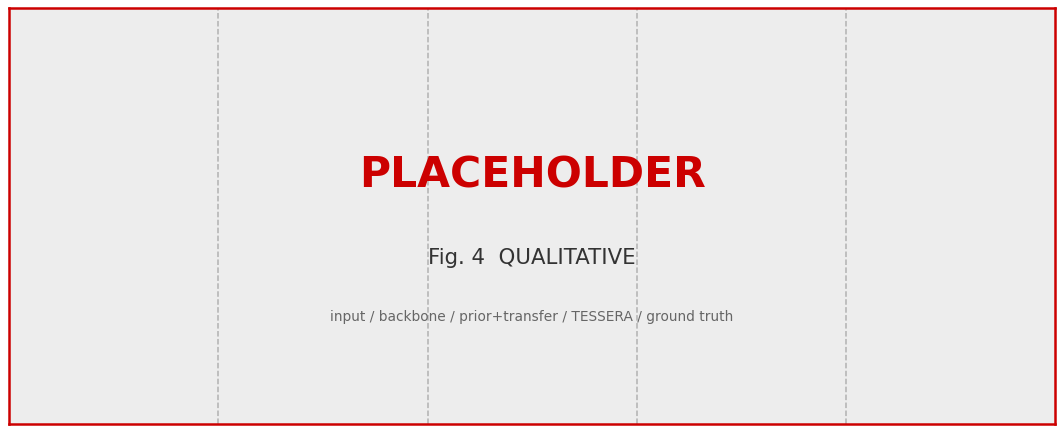
\includegraphics[width=0.66\textwidth]{qualitative.png}
  \caption{Renderings at held-out viewpoints. Columns: input, backbone,
       generative prior with transfer, TESSERA, ground truth. All share the
       same geometry; only the texture differs.}
  \label{fig:qualitative}
\end{figure}

\textbf{Earlier measurements.} Under a different protocol---a single frontal
view and a face-detector crop rather than the frame and facial-region mask of
Section~\ref{sec:protocol}---the backbone and the generative prior with
vertex-level transfer gave PSNR $13.74 \pm 1.71$ and $23.80 \pm 2.02$, SSIM
$0.447 \pm 0.031$ and $0.602 \pm 0.050$, LPIPS $0.513 \pm 0.040$ and
$0.350 \pm 0.087$ on the same \PH{74} subjects. These are not comparable with
Table~\ref{tab:main}: the full crop includes hair and background the mesh does
not represent, which inflates the difference between a partial and a complete
texture.

\textbf{Qualitative comparison.} Fig.~\ref{fig:qualitative} shows renderings at
held-out viewpoints. The backbone leaves regions without defined appearance
wherever the rendered viewpoint exposes surface that was occluded at capture.
Transferring a generative prior removes these regions but also replaces
observed detail with synthesized content in areas that were in fact
photographed. TESSERA retains the observed appearance and confines synthesized
content to the surface that neither observation nor symmetry covers.

\textbf{Predicted quality.} Evaluated against measured quality over all
subjects and all seven cameras, the rank correlation between $Q(\theta)$
(Eq.~\eqref{eq:vqp}) and PSNR, SSIM, LPIPS and CSIM is \PH{--}, \PH{--},
\PH{--} and \PH{--}. A prediction that tracks measured quality without access
to ground truth lets the representation report where it can be trusted, and in
an interactive capture setting indicates which additional view would contribute
most.

\begin{table}[htbp]
  \caption{Ablation on \PH{25} subjects, six held-out viewpoints.}
  \label{tab:ablation}
  \centering
  \begin{tabular}{@{}lcccc@{}}
    \toprule
    Variant & PSNR$\uparrow$ & SSIM$\uparrow$ & LPIPS$\downarrow$ & CSIM$\uparrow$ \\
    \midrule
    Vertex-level transport                & \PH{--} & \PH{--} & \PH{--} & \PH{--} \\
    w/o direct-evidence anchoring         & \PH{--} & \PH{--} & \PH{--} & \PH{--} \\
    w/o symmetry transport                & \PH{--} & \PH{--} & \PH{--} & \PH{--} \\
    w/o asymmetry correction              & \PH{--} & \PH{--} & \PH{--} & \PH{--} \\
    Single generative sample, $k=1$       & \PH{--} & \PH{--} & \PH{--} & \PH{--} \\
    Dilation and blurring in the atlas plane & \PH{--} & \PH{--} & \PH{--} & \PH{--} \\
    Surface adjacency, uniform anchoring  & \PH{--} & \PH{--} & \PH{--} & \PH{--} \\
    \textbf{Full}                         & \PH{--} & \PH{--} & \PH{--} & \PH{--} \\
    \bottomrule
  \end{tabular}
\end{table}

\textbf{Ablation.} Components are removed individually from the full method and
evaluated on a stratified sample of \PH{25} subjects over the six held-out
viewpoints (Table~\ref{tab:ablation}). \PH{[Per-component discussion, written
once measurements are available.]}

\textbf{Failure cases.} \PH{[Written from the measured results.]} We examine
the subjects with the lowest CSIM, group the failures by cause, and report what
fraction of them the reliability field identifies in advance, that is, whether
the worst subjects and viewpoints are also those for which $Q(\theta)$ is
lowest. Differences between TESSERA and the strongest competing method are
assessed with a paired Wilcoxon signed-rank test \cite{wilcoxon1945};
\PH{[result]}.

\section{Limitations}

\textbf{Inferred content remains inferred.} Where a region is neither observed
nor recoverable through symmetry, its appearance is supplied by the generative
prior and is plausible rather than correct. The reliability field marks these
regions, but marking is not correcting: the identity of the subject is not
recoverable there from a single image.

\textbf{Symmetry holds only approximately.} Because the correction of
Eq.~\eqref{eq:asym_correction} is restricted to low spatial frequencies, high
frequency features occurring on one side only, such as a mole or a scar, are
not reproduced on the occluded side. The estimated reliability
$\Rel_{\text{sym}}$ falls for subjects whose sides disagree and the fusion then
relies more heavily on the generative prior, so the failure is graceful; it is
nevertheless a failure to recover information that a second viewpoint would
provide directly.

\textbf{Appearance is static.} The completed atlas does not model
expression-dependent appearance such as the deepening of wrinkles or shifts in
specular highlights. Representations optimized per subject from video
\cite{gafni2021nerface,grassal2022nha,qian2024gaussianavatars,zhang2025fate}
capture these effects, at the cost of a video sequence and a per-subject
optimization stage. Extending the formulation to a small number of frames, with
observations accumulated over time, is a natural direction.

\textbf{Scope and dependencies.} Hair, clothing and accessories lie outside the
parametric surface and are absent from any texture defined on it, which is the
main reason we evaluate inside the facial region. Errors in the underlying
geometry propagate: the registration residual grows, $\Rel_{\text{geo}}$ falls,
and as the capture pose becomes more extreme the method degrades toward the
generative prior alone. Our measurements are taken under uniform studio
illumination with neutral expressions on a single dataset; behaviour under
unconstrained illumination, partial occlusion and stronger expressions remains
to be established, and we expect $\Rel_{\text{obs}}$ to require an explicit
treatment of shadowing in that setting.

\section{Conclusion}

We have argued that completing a face texture from a single image is better
posed as arbitration among sources of evidence than as image inpainting. The
argument rests on a simple observation: geometric transport, symmetry transport
and a generative prior each produce a residual in the course of their own
operation, and that residual estimates how far the evidence they supply can be
trusted. Because the three estimates share a scale and need no additional
supervision, the evidence can be combined in a single optimization rather than
selected by disjoint masks, and the generative prior can be placed last rather
than first.

TESSERA realizes this with a dense cross-topology transport map, an intrinsic
symmetry transport with a measured asymmetry correction, a per-texel
uncertainty from repeated sampling of the prior, and a reliability-anchored
Poisson problem on surface connectivity. On \PH{74} subjects at seven
calibrated viewpoints it \PH{[summary of the measured improvement]} relative to
the same prior applied conventionally, from a single image and with no
per-subject optimization. The reliability field is retained as part of the
output and predicts the quality attainable at a viewpoint before it is
rendered: a reconstructed appearance that reports where it is supported by
observation is more useful than one presenting inference and measurement as
though they were the same.

% ─────────────────────────────────────────────────────────────────────────────
\begin{credits}
\subsubsection{\discintname}
The authors have no competing interests to declare.
\end{credits}

\begin{thebibliography}{14}

\bibitem{paysan2009bfm}
Paysan, P., Knothe, R., Amberg, B., Romdhani, S., Vetter, T.: A 3D face model
for pose and illumination invariant face recognition. In: Proc. AVSS (2009)

\bibitem{feng2021deca}
Feng, Y., Feng, H., Black, M.J., Bolkart, T.: Learning an animatable detailed
3D face model from in-the-wild images. ACM Trans. Graph. \textbf{40}(4) (2021)

\bibitem{qian2024gaussianavatars}
Qian, S., Kirschstein, T., Schoneveld, L., Davoli, D., Giebenhain, S.,
Nie{\ss}ner, M.: GaussianAvatars: photorealistic head avatars with rigged 3D
Gaussians. In: Proc. CVPR (2024)

\bibitem{gafni2021nerface}
Gafni, G., Thies, J., Zollh\"ofer, M., Nie{\ss}ner, M.: Dynamic neural radiance
fields for monocular 4D facial avatar reconstruction. In: Proc. CVPR (2021)

\bibitem{grassal2022nha}
Grassal, P.-W., Prinzler, M., Leistner, T., Rother, C., Nie{\ss}ner, M.,
Thies, J.: Neural head avatars from monocular RGB videos. In: Proc. CVPR (2022)

\bibitem{zhang2025fate}
Zhang, J., et al.: FATE: full-head Gaussian avatar with textural editing from
monocular video. In: Proc. CVPR (2025)

\bibitem{li2024uvidm}
Li, H., Feng, Y., Xue, S., Liu, X., Zeng, B., Li, S., et al.: UV-IDM:
identity-conditioned latent diffusion model for face UV-texture generation.
In: Proc. CVPR, pp. 10585--10595 (2024)

\bibitem{blanz1999morphable}
Blanz, V., Vetter, T.: A morphable model for the synthesis of 3D faces.
In: Proc. SIGGRAPH (1999)

\bibitem{li2017flame}
Li, T., Bolkart, T., Black, M.J., Li, H., Romero, J.: Learning a model of
facial shape and expression from 4D scans. ACM Trans. Graph. \textbf{36}(6)
(2017)

\bibitem{rombach2022ldm}
Rombach, R., Blattmann, A., Lorenz, D., Esser, P., Ommer, B.: High-resolution
image synthesis with latent diffusion models. In: Proc. CVPR (2022)

\bibitem{duong2022vface}
Duong, H., Tran, T., Nguyen, V.B., Dao, V.A.: V-FACE: a large-scale Vietnamese
face image database in unconstrained environments. Int. J. iRobotics
\textbf{5}(2), 36--41 (2022)

\bibitem{zhang2018lpips}
Zhang, R., Isola, P., Efros, A.A., Shechtman, E., Wang, O.: The unreasonable
effectiveness of deep features as a perceptual metric. In: Proc. CVPR (2018)

\bibitem{wilcoxon1945}
Wilcoxon, F.: Individual comparisons by ranking methods. Biometrics Bull.
\textbf{1}(6), 80--83 (1945)

\bibitem{besl1992icp}
Besl, P.J., McKay, N.D.: A method for registration of 3-D shapes. IEEE Trans.
Pattern Anal. Mach. Intell. \textbf{14}(2), 239--256 (1992)

\end{thebibliography}

\end{document}
